\documentclass[onecolumn]{article}
%\usepackage{url}
%\usepackage{algorithmic}
\usepackage[a4paper]{geometry}
\usepackage{datetime}
\usepackage[margin=2em, font=small,labelfont=it]{caption}
\usepackage{graphicx}
\usepackage{mathpazo} % use palatino
\usepackage[scaled]{helvet} % helvetica
\usepackage{microtype}
\usepackage{amsmath}
\usepackage{subfigure}
\usepackage{hyperref}
\usepackage{graphicx}


\usepackage{listings}
\usepackage{color}
\definecolor{dkgreen}{rgb}{0,0.6,0}
\definecolor{gray}{rgb}{0.5,0.5,0.5}
\definecolor{mauve}{rgb}{0.58,0,0.82}

\lstset{frame=tb,
  language=python,
  aboveskip=3mm,
  belowskip=3mm,
  showstringspaces=false,
  columns=flexible,
  basicstyle={\small\ttfamily},
  numbers=none,
  numberstyle=\tiny\color{gray},
  keywordstyle=\color{blue},
  commentstyle=\color{dkgreen},
  stringstyle=\color{mauve},
  breaklines=true,
  breakatwhitespace=true,
  tabsize=2
}

% Letterspacing macros
\newcommand{\spacecaps}[1]{\textls[200]{\MakeUppercase{#1}}}
\newcommand{\spacesc}[1]{\textls[50]{\textsc{\MakeLowercase{#1}}}}

\title{\spacecaps{CENG 3521 Data Mining Assigment 2 }\\ \normalsize \spacesc{} }

\author{Gizem PESEN\\pesengizem@gmail.com}

%\date{\today\\\currenttime}


\begin{document}
\maketitle



\section{Contents }

\begin{itemize}
\item \hyperref[sec:1]{Declaration of Honor Code}
\item \hyperref[sec:2]{Single-layer Perceptron}
\item \hyperref[sec:2]{Classification task}
\item \hyperref[sec:2]{Visualization of decision boundary}
\item \hyperref[sec:2]{Multi-layer Perceptron}
\item \hyperref[sec:2]{Error convergence with multi-layer perceptron}
\end{itemize}

\section{Declaration of Honor Code}
\label{sec:1}
\textbf{Student ID :}170709050\\
\textbf{Name Surname:}Gizem Pesen\\

In the course of Data Mining (CENG 3521), I take academic integrity very seriously and ask
you to do as well. That’s why, this page is dedicated to some clear statements that defines
the policies of this assignment, and hence, will be in force. Before reading this assignment
booklet, please first read the following rules to avoid any possible violation on academic
integrity.

\begin{itemize}
\item This assignment must be done individually unless stated otherwise.
\item You are encouraged to discuss with your classmates about the given assignments, but
these discussions should be carried out in an abstract way. That is, you cannot copy
code (in whole or in part) of someone else, cannot share your code (in whole or in part)
with someone else either.
\item The previous rule also holds for the material found on the web as everything on the web
has been written by someone else.
• You must not look at solution sets o
\item You must not look at solution sets or program code from other years.
\item You cannot share or leave your code (in whole or in part) in publicly accessible areas.
\item You have to be prepared to explain the idea behind the solution of this assignment you
submit.
\item Finally, you must make a copy of your solution of this assignment and keep it until the
end of this semester.

\end{itemize}

\begin{figure}[ht!]
\centering
\includegraphics[width=10cm]{imza.png}
\end{figure}




\section{Single-layer Perceptron}
\label{sec:2}

\subsubsection{Classification task}
\label{sec:2}
\begin{lstlisting}[language=Python, caption= Imports] 
import time 
import warnings
from sklearn import metrics
from sklearn import model_selection 
warnings.filterwarnings("ignore")
from sklearn import linear_model #for linear regression
from sklearn.model_selection import train_test_split
from sklearn.datasets import make_classification #classification
import numpy as np #single layer neural network 
import matplotlib.pyplot as plt
from sklearn import svm, datasets
from sklearn.neural_network import MLPClassifier
from sklearn.preprocessing import StandardScaler
from sklearn.linear_model import Perceptron
from sklearn.metrics import classification_report,confusion_matrix
\end{lstlisting} 


It makes a lot of sense to define functions for tasks as in the solutions video of Assignment 1, and in this way I defined train and test into function. 

\begin{lstlisting}[language=Python, caption= Train and Test] 
def task1(sample_size,dimension_size,n_iter):
  X, y = make_classification(sample_size,dimension_size)
  X_train,X_test,y_train,y_test = model_selection.train_test_split(X,y, test_size=0.3,train_size= 0.7)
  #clf=linear_model.SGDClassifier(loss="log",max_iter=n_iter)
  #clf.fit(X_train,y_train)
\end{lstlisting} 

I used \textbf{Standard Scaler }from sklearn for  \textbf{Perceptron.}

\begin{lstlisting}[language=Python, caption= Standard Scaler] 
  scaler = StandardScaler()
  scaler.fit(X_train)
\end{lstlisting} 
\textbf{Scale (transform)} the training and the testing sets. Using the scaler that was fitted to \textbf{training data.}

\begin{lstlisting}[language=Python, caption= transform] 
  X_train_std = scaler.transform(X_train)
  X_test_std = scaler.transform(X_test)
\end{lstlisting} 

\begin{lstlisting}[language=Python, caption= select a subset of the features as before.] 
 np.unique(y)
  X_train_std =  X_train_std[:,[2,3]]
  X_test_std = X_test_std[:,[2,3]]
\end{lstlisting} 

\begin{lstlisting}[language=Python, caption= Perceptron] 
  ppn = Perceptron(max_iter=n_iter,eta0 =0.1)
  ppn.fit(X_train_std,y_train)
\end{lstlisting} 

\begin{lstlisting}[language=Python, caption= Calculation of error ] 
  #first I find error 
  y_predict = ppn.predict(X_test_std)
  error = metrics.mean_squared_error(y_test,y_predict)
  return error
'''
  #then I tried with accuracy score
  y_predict = ppn.predict(X_test_std)
  accuracy = accuracy_score(y_test,y_predict)*100
  return accuracy
  '''
\end{lstlisting} 

\subsubsection{Discussion}
\label{sec:2}

\begin{itemize}
\item As the number of tuples increases, the error rate decreases because there is more information.
\item As dimension increases, the error rate increases as the data size increases.
\item As the number of iterations increases, the error rate decreases.
\end{itemize}


\begin {tabular}{crrrrl}
\hline
Iteration &Tuple Size (m)& Dimension Size (n)  & Training Time (in ms))
& Error (cost)
  \\
\hline
  100&10,000
 &100&0.88&0.49\\
100&10,000
 &1,000&15.0&1.23\\
 100&100,000
&100&1.08&0.28\\ 100&250,000
&100&16.05&0.23\\ 
\hline
\end{tabular}
\\
\begin {tabular}{crrrrl}
\hline
Iteration &Tuple Size (m)& Dimension Size (n)  & Training Time (in ms))
& Error (cost)
  \\
\hline
 500 &10,000
 &100&1.08&0.26\\
500&10,000
 &1,000&1.50&0.32\\
 500& 100,000
&100&23.02&0.22\\ 500& 250,000
&100&27.03&0.13\\ 
\hline
\end{tabular}
\\

\subsubsection{Visualization of decision boundary}
\label{sec:2}

 .\\\\
 single-layer perceptron network on
solving a typical classification problem to visualize 3-D decision boundary.\\

 \begin{figure}[ht!]
\centering
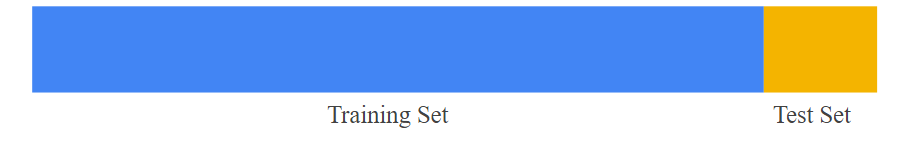
\includegraphics[width=7cm]{img1.png}
\end{figure}
.\\\\\\\\\\\\
\begin{lstlisting}[language=Python, caption= Visualization] 
 
  model = svm.SVC(kernel='linear')
  clf = model.fit(X, Y)
  z = lambda x,y: (-clf.intercept_[0]-clf.coef_[0][0]*x -clf.coef_[0][1]*y) /   clf.coef_[0][2]
  tmp = np.linspace(-5,5,30)
  x,y = np.meshgrid(tmp,tmp)
  fig = plt.figure()
  ax  = fig.add_subplot(111, projection='3d')
  ax.plot3D(X[Y==0,0], X[Y==0,1], X[Y==0,2],'ob')
  ax.plot3D(X[Y==1,0], X[Y==1,1], X[Y==1,2],'sr')
  ax.plot_surface(x, y, z(x,y))
  ax.view_init(30, 60)
  return plt.show()
\end{lstlisting} 
.\\
\subsubsection{Error convergence with multi-layer perceptron}
\label{sec:2}

\begin{lstlisting}[language=Python, caption= digits] 
  digits = datasets.load_digits()
\end{lstlisting} 

\begin{lstlisting}[language=Python, caption= MLPClassifier] 
  mlp = MLPClassifier(hidden_layer_sizes=(13,13,13),max_iter=500)
  mlp.fit(X_train,y_train)
  predictions = mlp.predict(X_test)
\end{lstlisting} 

\nocite{*}
\bibliographystyle{pl
\item 
\item ain}
\bibliography{references}
\end{document}
